\documentclass{./../div_teaching_slides}

\begin{document}
\title{ECON 340 \\ Economic Research Methods}
\author{Div Bhagia}
\date{Lecture 23 \\ Experiments \& Quasi-Experimental Methods}

%%%%%%%%%%%% 
\begin{frame}[noframenumbering, plain]
\maketitle
\end{frame}

%%%%%%%%%%%% 
\begin{frame}{It's hard to answer causal questions!}
\begin{witemize}
  \item Say, I am interested in whether going to college will increase Sam's income.
  \item Ideally, what I need: \\
  \begin{itemize}
  \normalsize
  \item Income of Sam if he goes to college \\
  \item Income of Sam if he does not go to college \\~\\
\end{itemize}
But a Sam with and without college doesn’t exist! \\~\\
Hence, this is a situation of a missing \textit{counterfactual}. 
\end{witemize}
\end{frame}

%%%%%%%%%%%% 
\begin{frame}{What's the counterfactual?}
Suppose Sam does not end up going to college. \\~\\ 

Can we answer what would happen if he did?
$$ \underbrace{Income_{Sam,college=1}}_{\text{Missing counterfactual}}-Income_{Sam, college=0} $$
What can we do? Is there a good proxy for the counterfactual outcome? \\~\\
\pause We want someone just like Sam, who went to college. 
\end{frame}

%%%%%%%%%%%% 
\begin{frame}{Randomization}
\begin{witemize}
  \item Gold standard: \textit{Randomized controlled trials} (RCTs) or \textit{experiments}
  \item Common in medicine and sciences, limited in social sciences
  \item Assign \textit{treatment} randomly, then on average individuals in the \textit{treated} group similar to individuals in the \textit{control} group
   \end{witemize}
\end{frame}

\begin{frame}{Randomized controlled trials}
Define, $$D =  \begin{cases}
  	1 \quad \text{if received treatment} \\
  	0 \quad \text{if did not receive treatment} \\
  \end{cases} $$ \\~\\
Outcome:
$$ Y = \beta_0 + \beta_1 D + u , \quad \quad E(u)=0 $$ \\~\\
If $D$ is randomized, the exogeneity assumption is satisfied:
$$ E(u|D=1) = E(u|D=0) =0$$
\end{frame}

%%%%%%%%%%%% 
\begin{frame}{Treatment Effect}
$$ Y = \beta_0 + \beta_1 D + u $$ \\~\\
Under exogeneity $E(u|D)=0$, the difference in the dependent variable between individuals is due to $D$: \\
$$ TE =  E(Y|D=1)-E(Y|D=0) = \beta_1 $$ \\
\vspace{1em}
This effect is called the treatment effect (TE). \\~\\
\end{frame}

%%%%%%%%%%%% 
\begin{frame}{Example}
\vspace{-0.5em}
\begin{witemize}
  \item 300 individuals participated in an RCT to evaluate the effect of caffeine on sleep.
  \item Treatment: $$D =  \begin{cases}
  	1 \quad \text{if given a cup of caffeinated coffee before bed} \\
  	0 \quad \text{if given a cup of decaf coffee before bed} \\
  \end{cases} $$ 
  \item Flipped a coin to decide which individuals got the real coffee vs decaf (\textit{placebo})
  \item Measure the quality of sleep using a score \\~\\
\end{witemize}
Aside: Should the control group get decaf or no coffee?
\end{frame}

%%%%%%%%%%%% 
\begin{frame}{Example}
\vspace{-1em}
$$ Sleep Score = \beta_0 + \beta_1 D + u , \quad \quad E(u)=0 $$ \\~\\
\begin{witemize}
  \item We expect different individuals to have different sleep scores due to several factors, which is captured by $u$
  \item But since we randomized treatment, these factors are uncorrelated with treatment, i.e., $E(u|D)=E(u)$ or equivalently $Cov(D,u)=0$.
  \item In other words, some individuals may sleep poorly, but there is an equal chance for these individuals to end up in the treatment or the control group
\end{witemize}
\end{frame}

%%%%%%%%%%%% 
\begin{frame}{Example}
\vspace{-1em}
$$ Sleep Score = \beta_0 + \beta_1 D + u , \quad \quad E(u)=0 $$ \\
\begin{witemize}
  \item With randomization, it is no longer the case that individuals who had the real coffee might be systematically different from those who didn't 
  \item Hence, the difference in outcomes between the two groups captures the impact of coffee on sleep and not the omitted factors that affect sleep and are correlated with coffee consumption. 
 \end{witemize}
\end{frame}

%%%%%%%%%%%%%%%%%%%%
\begin{frame}{A Simple Example}
\begin{witemize}
  \item Say half of the people are good sleepers with $u=10$, while the other half are poor sleepers with $u = -10$
  \item We randomly put half of the individuals into the control group and half into the treatment group
  \item Then we should expect a 50-50 distribution of good and poor sleepers in both treatment and control groups
  $$ E(u|D=1) = 0.5(10) + 0.5(-10) = 0 $$
  $$ E(u|D=0) = 0.5(10) + 0.5(-10) = 0 $$
\end{witemize}
\end{frame}

%%%%%%%%%%%%%%%%%%%%
\begin{frame}{Randomization}
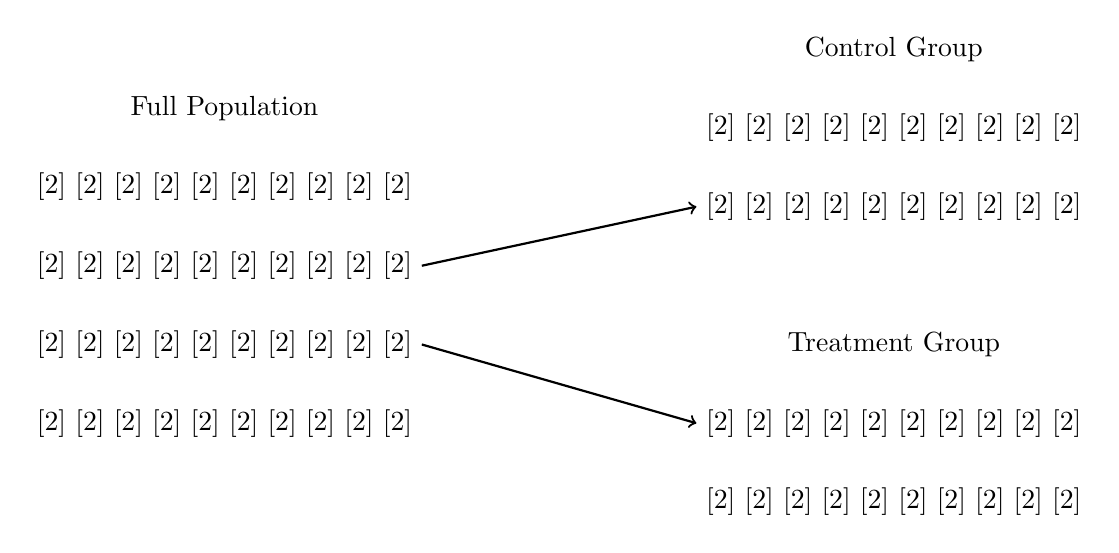
\begin{tikzpicture}
%%%%%%% Full Population
\node (pop_text) {Full Population};
\node (pop_row1) [below of=pop_text] {\purple{\Strichmaxerl[2]} \ddgrey{\Strichmaxerl[2]} \purple{\Strichmaxerl[2]} \ddgrey{\Strichmaxerl[2]} \purple{\Strichmaxerl[2]} \ddgrey{\Strichmaxerl[2]} \purple{\Strichmaxerl[2]} \ddgrey{\Strichmaxerl[2]} \purple{\Strichmaxerl[2]}  \ddgrey{\Strichmaxerl[2]} };
\node (pop_row2) [below of=pop_row1] {\purple{\Strichmaxerl[2]} \ddgrey{\Strichmaxerl[2]} \purple{\Strichmaxerl[2]} \ddgrey{\Strichmaxerl[2]} \purple{\Strichmaxerl[2]} \ddgrey{\Strichmaxerl[2]} \purple{\Strichmaxerl[2]} \ddgrey{\Strichmaxerl[2]} \purple{\Strichmaxerl[2]}  \ddgrey{\Strichmaxerl[2]} };
\node (pop_row3) [below of=pop_row2] {\purple{\Strichmaxerl[2]} \ddgrey{\Strichmaxerl[2]} \purple{\Strichmaxerl[2]} \ddgrey{\Strichmaxerl[2]} \purple{\Strichmaxerl[2]} \ddgrey{\Strichmaxerl[2]} \purple{\Strichmaxerl[2]} \ddgrey{\Strichmaxerl[2]} \purple{\Strichmaxerl[2]}  \ddgrey{\Strichmaxerl[2]} };
\node (pop_row4) [below of=pop_row3] {\purple{\Strichmaxerl[2]} \ddgrey{\Strichmaxerl[2]} \purple{\Strichmaxerl[2]} \ddgrey{\Strichmaxerl[2]} \purple{\Strichmaxerl[2]} \ddgrey{\Strichmaxerl[2]} \purple{\Strichmaxerl[2]} \ddgrey{\Strichmaxerl[2]} \purple{\Strichmaxerl[2]}  \ddgrey{\Strichmaxerl[2]} };
%%%%%%% Control Group
\node (ct_text) [left of=pop_text, xshift=9.5cm, yshift=0.75cm] {Control Group};
\node (ct_row1) [below of=ct_text] {\purple{\Strichmaxerl[2]} \ddgrey{\Strichmaxerl[2]} \purple{\Strichmaxerl[2]} \ddgrey{\Strichmaxerl[2]} \purple{\Strichmaxerl[2]} \ddgrey{\Strichmaxerl[2]} \purple{\Strichmaxerl[2]} \ddgrey{\Strichmaxerl[2]} \purple{\Strichmaxerl[2]}  \ddgrey{\Strichmaxerl[2]} };
\node (ct_row2) [below of=ct_row1] {\purple{\Strichmaxerl[2]} \ddgrey{\Strichmaxerl[2]} \purple{\Strichmaxerl[2]} \ddgrey{\Strichmaxerl[2]} \purple{\Strichmaxerl[2]} \ddgrey{\Strichmaxerl[2]} \purple{\Strichmaxerl[2]} \ddgrey{\Strichmaxerl[2]} \purple{\Strichmaxerl[2]}  \ddgrey{\Strichmaxerl[2]} };
%%%%%%% Treatment Group
\node (tr_text) [below of=ct_row2, yshift=-0.75cm]{Treatment Group};
\node (tr_row1) [below of=tr_text] {\purple{\Strichmaxerl[2]} \ddgrey{\Strichmaxerl[2]} \purple{\Strichmaxerl[2]} \ddgrey{\Strichmaxerl[2]} \purple{\Strichmaxerl[2]} \ddgrey{\Strichmaxerl[2]} \purple{\Strichmaxerl[2]} \ddgrey{\Strichmaxerl[2]} \purple{\Strichmaxerl[2]}  \ddgrey{\Strichmaxerl[2]} };
\node (tr_row2) [below of=tr_row1] {\purple{\Strichmaxerl[2]} \ddgrey{\Strichmaxerl[2]} \purple{\Strichmaxerl[2]} \ddgrey{\Strichmaxerl[2]} \purple{\Strichmaxerl[2]} \ddgrey{\Strichmaxerl[2]} \purple{\Strichmaxerl[2]} \ddgrey{\Strichmaxerl[2]} \purple{\Strichmaxerl[2]}  \ddgrey{\Strichmaxerl[2]} };
%%%%%%%%% Arrows
\draw[->, thick] (pop_row2.east) --  (ct_row2.west) {};
\draw[->, thick] (pop_row3.east) -- (tr_row1.west) {};

\end{tikzpicture}
\end{frame}



%%%%%%%%%%%% 
\begin{frame}{Experiments are not always feasible}
\begin{witemize}
  \item It's often infeasible to run experiments to answer interesting economic questions. We can't just randomize college attendance for a group of individuals!
  \item Economists have to be clever. Use \textit{quasi}-experimental variation. Need to look for \textit{natural experiments}.
  \item \href{https://www.nobelprize.org/prizes/economic-sciences/2021/press-release/}{2021 Nobel Prize} awarded to David Card, Joshua Angrist and Guido Imbens for their contributions to quasi-experimental methods in economics. (Reading on course website)
\end{witemize}
\end{frame}

%%%%%%%%%%%%
\begin{frame}{Angrist and Krueger (1991)}
\begin{witemize}
  \item In the US, children typically enter school in the fall of the year they turn six 
  \item Individuals are required by law to stay in school until their sixteenth birthday
  \item Because all children who are born in a particular calendar year start school on the same date, children who are born early in the year can leave school sooner than children born later in the year.
\end{witemize}
\end{frame}

%%%%%%%%%%%%
\begin{frame}{Angrist and Krueger (1991)}
Example: \\
\begin{witemize}
  \item Sam born in Jan 1991, starts school in Aug 1997, can drop in Jan 2007
  \item Jack born in Dec 1991, starts school in Aug 1997, can drop in Dec 2007 
\end{witemize}
Jack can drop out almost a year earlier out of school than Sam, just because he was born in Dec rather than Jan. \\~\\
As long as the quarter of birth is random, which is plausible, we could use this variation to estimate the causal impact of education on income. 
\end{frame}

\begin{frame}{Angrist and Krueger (1991)}
\centering
\includegraphics[scale=0.34]{angrist-krueger.png}
\end{frame}

%%%%%%%%%%%%
\begin{frame}{Quasi-Experimental Methods}
There is a growing toolkit of quasi-experimental methods. Here are three popular ones: \\~\\
\begin{witemize}
 \item[(1).] \textit{Propensity Score Matching:} {Match individuals in the treatment group with individuals in the control group who are similar in all relevant characteristics except for the treatment.}
 \end{witemize}
\end{frame}

%%%%%%%%%%%%
\begin{frame}{Quasi-Experimental Methods}
There is a growing toolkit of quasi-experimental methods. Here are three popular ones: \\~\\
\begin{witemize}
  \item[(2).] \textit{Regression Discontinuity:} This design is used when an intervention is assigned based on a continuous score or threshold, and participants on either side of the threshold are assumed to be similar except for the treatment. The difference in outcomes between the two groups is used to estimate the causal effect of the treatment.
 \end{witemize}
\end{frame}

%%%%%%%%%%%%
\begin{frame}{Londo\~{n}o-V\'{e}lez et. al. (2024)}
\begin{witemize}
  \item In 2014, Colombia implemented a nationwide financial aid program covering the tuition of four-year undergraduate programs at 33 ``high-quality'' universities
  \item Beneficiaries required to satisfy two conditions: (1) score in the top decile of Colombia’s national standardized high school exit exam, SABER 11, and (2) come from households in the poorest 52.8\%
  \item Leverage the program’s discontinuous assignment rules based
on test scores and household wealth using a regression discontinuity design
\end{witemize}

\end{frame}
%%%%%%%%%%%%
\begin{frame}{Eligibility}
\includegraphics[scale=0.475]{rd1.png}
\end{frame}

%%%%%%%%%%%%
\begin{frame}{Share enrolling in college}
\includegraphics[scale=0.55]{rd2.png}
\end{frame}


%%%%%%%%%%%%
\begin{frame}{Quasi-Experimental Methods}
There is a growing toolkit of quasi-experimental methods. Here are three popular ones: \\~\\
\begin{witemize}
  \item[(3).] \textit{Differences-in-Difference:} This design estimates the causal effect of an intervention by comparing the change in outcomes between a treatment group and a control group over time, assuming similar trends in the absence of the intervention.
 \end{witemize}
\end{frame}

%%%%%%%%%%%%
\begin{frame}{Differences-in-Differences}
\centering
\includegraphics[scale=0.3]{dd.png}
\end{frame}


\end{document}